%%%%%%%%%%%%%%%%%%%%%%%%%%%%%%%%%%%%%%%%%%%%%%%%%%%%%%%%%%%
% EPFL report package, main thesis file
% Goal: provide formatting for theses and project reports
% Author: Mathias Payer <mathias.payer@epfl.ch>
%
% To avoid any implication, this template is released into the
% public domain / CC0, whatever is most convenient for the author
% using this template.
%
%%%%%%%%%%%%%%%%%%%%%%%%%%%%%%%%%%%%%%%%%%%%%%%%%%%%%%%%%%%
\documentclass[a4paper,11pt,oneside]{report}
% Options: MScThesis, BScThesis, MScProject, BScProject
\usepackage[BScThesis,lablogo]{EPFLreport}
\usepackage{xspace}
\usepackage{textcomp}
\usepackage{indentfirst}
\usepackage{float}
\usepackage{tikz}

\title{A Binary Rewriter Benchmarking Tool}
\author{Khalil M'hirsi}
\supervisor{Luca Di Bartolomeo}
\adviser{Prof. Dr. sc. ETH Mathias Payer}
%\coadviser{Second Adviser}
%\expert{The External Reviewer}

\newcommand{\sysname}{FooSystem\xspace}

\begin{document}
\maketitle

\begin{abstract}
    \setlength{\parindent}{4em}
    Binary rewriters, critical tools for software analysis, transformation, and security,
    necessitate comprehensive and efficient evaluation methodologies to ensure their
    effectiveness and reliability. This task becomes a challenge due to the complexity and
    diversity of real-world applications, the subtle changes a rewriter can introduce, and the
    intricate balance between comprehensive evaluation and performance efficiency. This work
    introduces a novel tool designed to address the challenge of effectively testing binary
    rewriters. Our tool improves both the convenience and efficiency of this testing process by
    automating key aspects and introducing a streamlined approach to data collection and
    analysis. It not only saves valuable time and resources but also enhances the precision of the
    testing process by minimizing human error and providing a systematic, repeatable process
    for evaluating binary rewriters.

    The tool's flexible architecture allows it to be adapted for testing a broad spectrum of
    rewriters, binary subjects and architectures, thus potentially benefiting a wide range of
    applications in software development, maintenance, and security. Through rigorous testing
    and case studies, we demonstrate the tool's robust performance and its potential to
    advance the field of binary rewriting. This work is expected to serve as a significant
    contribution towards facilitating more effective, efficient, and user-friendly testing of binary
    rewriters, and in turn, supporting the development of more reliable and secure software
    systems.
\end{abstract}

\maketoc

%%%%%%%%%%%%%%%%%%%%%%
\chapter{Introduction}
%%%%%%%%%%%%%%%%%%%%%%

\setlength{\parindent}{4em}
Binary rewriting is a field in software engineering that deals with the alteration of
binary code, which is the primary, executable format of software. Unlike source code, which
is written in high-level languages and is intended for human understanding, binary code
consists of machine code, the lowest level of programming, which is natively executable by
the computer's processor.

Binary rewriters, as the name suggests, are tools that manipulate binary code. They
parse the binary executable, understand its structure and semantics, and then modify it,
generating a new binary that retains the functionality of the original program while
incorporating new characteristics or enhancements. The binary rewriting technique is
leveraged in many computer science domains due to its ability to modify programs without
needing access to their source code.

One primary usage of binary rewriters is in the field of software security. They are
used for injecting mitigations in compiled programs, such as control-flow integrity or
memory sanitization. By rewriting the binary, it's possible to add these security features
even if the source code is not available, making them a valuable tool in hardening third-
party software or legacy systems. Binary rewriters also play a crucial role in software
performance optimization. They can apply performance improvement strategies, like
profile-guided optimizations, to the binaries of applications. Furthermore, binary rewriters
can be used for porting software to different hardware or software platforms, by replacing
platform-specific instructions or system calls. Additionally, they are extensively used in the
field of reverse engineering for program analysis and understanding. Binary rewriters can
add instrumentation to the binary code that logs useful runtime information, helping to
understand the program's behavior.

Despite their wide-ranging applications, binary rewriting is a challenging process due
to the complexity of interpreting machine code accurately, handling indirect jumps and
calls, dealing with dynamic linking and loading, among other hurdles.

While binary rewriters have significant potential in various applications, their
effectiveness and reliability are often unverified or assumed based on limited case studies.
Given the complex nature of binary rewriting and the multitude of challenges it involves, the
need for a comprehensive, efficient, and convenient tool to test binary rewriters cannot be
overstated.

A core issue is that currently, there isn't a standardized methodology for evaluating
the performance of binary rewriters across different use cases and conditions. While several
tools already exist for binary rewriting as mentioned above, their evaluation often happens
in isolation, utilizing different benchmarks and criteria that may not reflect the broad range
of scenarios encountered in real-world applications.

In light of this, the existing testing methodologies tend to focus on the depth of
testing on a small sample size rather than a breadth-first approach. As a result, they might
not fully capture the variety and diversity of real-world use cases. In other words, there is a
lack of extensive testing on a wide array of programs that reflect the range of applications
that might be encountered in a practical setting.

The highlighted issues accentuate the demand for a tool that integrates a uniform
benchmarking system for assessing binary rewriters, while simultaneously guaranteeing a
testing process that is comprehensive, scalable, and mirrors real-world scenarios. An
example of a study pivoting towards such a breadth-first approach (incorporating a large
number of subjects with fewer, but targeted, tests) is GrammaTech’s “Binary Lifter
Evaluation.” While this study marks a significant step forward, it also opens up discussions
around further improvements. The effectiveness of their testing criteria, the practicality of
the test suite, and the broadness of their coverage could be further explored and optimized
to establish a balance between the range of test subjects and depth of the evaluation.
Therefore, their work should be seen as a valuable foundation upon which further
advancements in the field can be built.

The subsequent sections will introduce RBMT, our new tool designed to test binary
rewriters effectively and efficiently, contributing to their development and refining process.
By providing a convenient and systematic approach to test these vital tools, we aim to
facilitate their ongoing advancement and their ability to shape a more secure and efficient
software landscape.

%%%%%%%%%%%%%%%%%%%%
\chapter{Background}
%%%%%%%%%%%%%%%%%%%%
\setlength{\parindent}{4em}
Binary rewriting is a technique that allows modifications to be made directly to
compiled binary executables. The process involves analyzing and potentially altering a
binary without having access to its source code. This is a powerful approach that can be
used in several applications such as software testing, debugging, optimization, obfuscation,
and reverse engineering. It also plays a significant role in the domain of software security,
where it can be used for purposes like malware analysis and defense, software hardening,
and vulnerability patching.

Rewriting techniques can broadly be classified into two categories: static and
dynamic. Static rewriting is performed offline, i.e., the binary is modified before it is loaded
for execution. This type of rewriting involves transforming the entire binary, creating a new
version that can be executed independently of the original binary. On the other hand,
dynamic binary rewriting is performed on-the-fly during the execution of a binary. This type
of rewriting gives the flexibility to change the behavior of the program at runtime, which can
be highly valuable in cases such as profiling, instrumentation, and real-time security
defense.

Despite its potential, binary rewriting presents a number of challenges. Firstly, due
to the high complexity of binary code and the absence of high-level semantic information,
analyzing and accurately rewriting binaries is a complex task. The challenge becomes more
severe when dealing with indirect control flow transfers (such as function pointers or virtual
calls in object-oriented languages), which are not statically analyzable. Secondly, ensuring
the semantic equivalence between the original and rewritten binary is non-trivial,
particularly when aggressive optimizations are applied. Thirdly, the rewriting process itself
should be efficient in terms of both time and space to avoid introducing significant
overhead.

Over the years, numerous binary rewriting tools have emerged, each characterized
by distinct strengths and weaknesses. Tools such as Zipr, DDisasm, and Retrowrite
concentrate on delivering robust static rewriting capabilities. In contrast, others, such as
QEMu, enable dynamic binary instrumentation functionalities.

The efficacy of these tools can be constrained by various factors. These encompass
the intricacy of the binary code, the unique architectural attributes of the target system,
and the level of resilience necessitated by the application in question. For instance, static
rewriters like Zipr and DDisasm excel in contexts where full binary transformation is
required prior to execution. However, handling binaries with complex code structures or
ensuring precise semantic equivalence between original and rewritten binaries could pose
challenges. On the other hand, QEMu's dynamic binary instrumentation comes to the fore in
scenarios that require real-time modifications during program execution, though it may be
constrained by runtime performance overheads.

Despite substantial advancements in the field of binary rewriting, the need for more
sophisticated tools and techniques remains to enable more accurate and efficient binary
rewriting processes. The reason being, binary rewriting caters to a wide array of applications
from malware analysis to software hardening and from performance optimization to real-
time defense mechanisms. Therefore, any innovation in this domain can trigger
transformative impacts across the broader software industry, leading to improved software
reliability, security, and efficiency.

One significant contribution in the binary rewriting domain was made by
GrammaTech. Founded in 1988 as a technology spin-off from Cornell University,
GrammaTech is a well-established software-development tools vendor based in Bethesda,
Maryland, with a research center in Ithaca, New York. The company provides application
security testing products and software research services, making substantial strides in the
software engineering domain. Among their numerous endeavors, their work on "Binary
Lifter Evaluation" stands out. This paper aimed to test the generality, reliability, and
performance of binary rewriters and the binaries they produce.

In their study, GrammaTech utilized 10 different static rewriters such as Zipr,
ddisasm, e9patch, and Retrowrite, to recompile 3344 binaries sourced from 34 benchmark
programs and three production compilers. They adopted a breadth-first approach, focusing
on incorporating a large number of subjects with fewer, yet significant tests. While this
research marked a significant step in the field, it revealed some inherent challenges in their
methodology. Their quest to cover a vast range of test subjects may have inadvertently
compromised the depth of their evaluation. Thus, the study's effectiveness, comprehensive
nature, usability, and real-world applicability of their testing criteria and test suite could be
further enhanced.

This gap in the binary rewriter testing domain triggered the motivation behind our
project: developing a robust benchmarking tool for binary rewriters, capable of delivering a
thorough, real-world-reflective, and scalable testing process. By offering a more balanced,
comprehensive, and efficient approach to binary rewriter testing, our tool aims to set a
uniform standard for binary rewriter evaluation. The subsequent sections will introduce our
novel tool, the Rewriter Bench Marking Tool (RBMT), designed to overcome the existing
limitations and bridge the gap in binary rewriter testing.

%%%%%%%%%%%%%%%%
\chapter{Challenges}
%%%%%%%%%%%%%%%%

\setlength{\parindent}{4em}
Embarking on the journey of developing a binary rewriter testing tool, we inevitably
face a unique set of challenges. Our work parallels GrammaTech's "Binary Lifter Evaluation"
in many ways, allowing for valuable comparisons and insights. Analyzing the challenges
encountered by GrammaTech's ambitious project can inform and guide our own
development process.

The primary goal, as per our understanding of GrammaTech's work, is to test the
generality, reliability, and performance of binary rewriters and the binaries they produce.
The challenge lies not only in achieving these objectives but in doing so in a way that reflects
a diverse set of real-world scenarios. The binary rewriter testing tool must be able to handle
a vast range of binaries and test across different compilers, architectures, and code
complexities.

The task of creating such a comprehensive and representative test suite is a daunting
one. The test suite must not only be vast and diverse but also needs to be effectively
manageable and easily scalable. Further challenges will be discussed as we delve into the
specifics of our proposed solution and its design methodology. Through this discourse, we
aim to not only highlight the challenges that we face but also to propose potential solutions.

\textbf{Diversity and Generality of Testing}

One of the primary challenges faced in the development of a binary rewriter testing
tool is ensuring that it accurately reflects a broad spectrum of real-world scenarios.
GrammaTech's methodology focused on breadth rather than depth, implying an attempt to
test many programs instead of extensive testing on a small sample size. However, the binary
rewriter testing tool must have a comprehensive suite of tests to handle a diverse set of
binaries. The challenge is in ensuring the test suite's representativeness and generality,
enabling it to test across different compilers, architectures, operating systems and code
complexity.

\textbf{Evaluation Metrics and Benchmarks}

Choosing the right evaluation metrics for a binary rewriter testing tool is a significant
challenge. GrammaTech's approach considers both functional and non-functional metrics.
While these metrics offer crucial information about the functionality and performance of
the rewritten binaries, there is an ongoing discussion about whether these metrics
holistically measure the generality and reliability of the rewriters and the binaries they
produce.

The functional metrics employed in GrammaTech's study, namely the Null Function
Test and the AFL Function Test, provide an initial understanding of the rewriter's ability to
produce functional binaries. However, these tests may not fully capture the richness and
diversity of real-world scenarios. They indicate whether the rewriters can produce
functional binaries under a controlled set of conditions, but the real-world use cases might
pose far more varied and complex challenges. Factors such as how the rewritten binary
interacts with different operating systems, handles varying loads, or reacts to a spectrum of
input data, are not fully assessed in these tests.

The study also incorporated non-functional metrics to gauge the performance and
efficiency of the rewriters, including their runtime, memory usage, and changes in file size.
Although these metrics are important for evaluating performance, they may not be directly
indicative of the rewriters' reliability and generality. A rewriter may exhibit high efficiency
but might struggle with maintaining the exact functionality of complex binaries.

A notable part of the evaluation process is the set of tasks and checkpoints defined
by GrammaTech. They include NOP (successful rewrite with no modifications), AFL
(successful rewrite with modifications that support AFL++ instrumentation), and various
checkpoints like IR (Intermediate result is collectable), EXE (successful generation of new
executable), and AFL EXE (successful generation of AFL Instrumented exec).

These tasks and checkpoints provide a structured framework to evaluate the binary
rewriters. However, they raise questions about their comprehensiveness and
representativeness. Is the successful generation of an AFL Instrumented executable a strong
enough indicator of the rewriter's effectiveness in real-world scenarios? Are the tasks and
checkpoints sufficient and comprehensive to assess the wide range of capabilities that real-
world applications demand from binary rewriters?

Furthermore, the study's test suite included 34 different applications and use cases.
Although this provided 3344 binaries for testing, it is worth questioning if this sample size
and selection is adequately representative of real-world applications.

These considerations underscore the challenge of developing a comprehensive and
representative test suite and highlight the need for carefully chosen evaluation metrics. Our
aim is to address these issues and present a more robust, real-world reflective, and holistic
evaluation approach for binary rewriters.

\textbf{Scalability and usability of the test suite}

A key challenge in the creation of a binary rewriter testing tool is the development of
a test suite that is not only diverse and representative, but also scalable and user-friendly.
For the testing tool to be practical and widely usable, the test suite must be designed to
operate smoothly on a wide range of computer systems.

The usability of the test suite is paramount. The test suite must be clear and
intuitive, allowing users, regardless of their level of technical expertise, to run and interpret
the tests. It should also be designed with future updates and expansions in mind. This
ensures the testing tool remains relevant and adaptable to evolving needs and
advancements in binary rewriting techniques.

Accessibility is another vital consideration. Unlike GrammaTech's private repositories
in their "lifter-eval" project, the test suite and its associated resources should be openly
accessible to users. This transparency not only enhances usability but also encourages
collaboration and contribution from the wider community, thereby strengthening the
robustness and comprehensiveness of the tests.

Modularity is a key design principle that enhances the versatility of the test suite. A
modular design allows users to execute a subset of tests as needed, providing the flexibility
to focus on specific areas of interest or concern. This is particularly beneficial during
debugging processes, where isolating specific functionalities can greatly expedite problem
identification and resolution.

Furthermore, the test suite should be designed to leverage caching capabilities
where possible. Effective use of caching can dramatically speed up repeated tests by storing
and reusing previously computed results. This is especially valuable in a testing
environment, where iterations are frequent and any reduction in computation time can
significantly streamline the testing process.

In essence, designing a test suite that embodies these principles is challenging, yet it
forms a cornerstone of creating a powerful, usable, and resilient binary rewriter testing tool.
The test suite must be representative and comprehensive, but it must also be user-friendly,
scalable, modular, and efficient, thus facilitating wide adoption and usage. Through our
endeavor, we aim to address these challenges and create a binary rewriter testing tool that
meets these stringent requirements.

%%%%%%%%%%%%%%%%%%%%%%%%
\chapter{Design}
%%%%%%%%%%%%%%%%%%%%%%%%

\setlength{\parindent}{4em}
\textbf{Grammatech’s testsuite}

The initial phase of our project design involved leveraging GrammaTech's lifter
evaluation repository as a foundation. We allocated three weeks to this endeavor, hoping to
benefit from the existing infrastructure as stated in GrammaTech's declaration:

"All artifacts generated in this work, including our evaluation infrastructure, corpus
of test binaries, predictive models, and the evaluated tools, are publicly available at:\\
https://gitlab.com/GrammaTech/lifter-eval (GrammaTech, n.d.)."

Our strategy was to meticulously adhere to the available documentation for
constructing each docker image using the provided Dockerfiles. Unfortunately, this
endeavor proved less fruitful than expected.

The primary issues arose from private repositories for tools and subjects, which
rendered them inaccessible. Additionally, the Dockerfiles were outdated, resulting in
crashes during attempts to download specific binaries and files. The absence of
comprehensive documentation only added to these problems.

Even after successfully building docker images, they lacked crucial packages
necessary to run their tool command. This suggested a significant portion of the work was
outdated. However, it is noteworthy that throughout the semester, GrammaTech has been
actively improving their repository, implementing new features and adding more binaries to
the test suite, including new languages like Fortran and Ocaml.

This initial setback underscored the importance of adaptability in our design
strategy, leading us to pivot towards developing our own infrastructure for the project. We
will nevertheless mention that having been able to build a few important docker images
using Grammatech’s repository, we saved time in not needing to build the tools required to
rewrite binaries. The tools that were salvaged in this manner were Zipr, e9patch, and
GrammaTech’s own rewriter ddisasm.

\textbf{Building our custom pipeline}

With the complexities associated with this expansive project and the potential
challenges of constructing a robust and comprehensive test suite, we had to adjust our
strategy when constructing our own pipeline. Given that I was the sole architect of this
project, it was critical to ensure the feasibility of each development stage.

Our approach mirrored the principles of Rapid or Agile development, whereby we
established tangible, weekly goals to ensure continuous progression. The primary objective
was to accelerate the delivery of a Minimum Viable Product (MVP) and subsequently
enhance its functionality by incorporating as many desired features as possible over time.
This strategic planning not only ensured the project's success rate but also addressed the
earlier-mentioned challenges of scalability and modularity.

In terms of the operating system, we decided to restrict the test suite to Linux for
the initial development phase. This decision was driven by the ease of scripting on Linux and
the convenience of automating and instrumenting installations of the test subjects from
source. While our code and scripts needed to maintain simplicity, even if it occasionally
required 'hacky' solutions, this was necessary to ensure the pipeline's internals remained
understandable and easily modifiable. This is a major difference from Grammatech’s over-
engineered tool pipeline.

Communication within our pipeline was primarily facilitated through file exchanges
on the Linux file system, leveraging another strength of the UNIX-based OS. By focusing on
simplicity and agility in our design strategy, we aimed to build a pipeline that was, above all
else, both efficient and adaptable to future enhancements.

\textbf{Tool Architecture and initiating the Testing Pipeline}

Our new benchmarking tool, imaginatively dubbed the Rewriter Benchmarking Tool
(RBMT), was designed to utilize comprehensive and trusted test suites from popular
software. The RBMT was conceived with the primary objective of comparing the
performance of binaries, pre- and post-rewrite, using various binary rewriters derived from
GrammaTech's work.

The initial development phase entailed the creation of scripts to facilitate the
efficient management of docker containers. These scripts enabled one-command
installation, saving, and updating of the docker images, including dependency installations,
which we will discuss shortly.

One constant challenge that persisted throughout the project was the need to rely
on these 'black box' docker images. These were established early in the project when we
were still familiarizing ourselves with the nuances of developing in a remote Linux server
environment and learning to use tools like Docker. The docker images' sole purpose was to
facilitate the running of rewriting tools.

In retrospect, it would have been more efficient to create our Dockerfiles to enable
more effective storage and updating of these images, given their central role in the test
suite's development. The necessity for our own Dockerfiles arises from two primary
considerations. First, ensuring the availability of the 'sudo' command within the docker
environments. Second, segregating the workspace into three separate directories based on
the tool name (\textless{}tool\_name\textgreater{}-wd) ensured that running the three different tools did not
interfere with each other due to the Linux permission system.

With the capability to rewrite any binary file using three different rewriters
confirmed, we turned our attention to constructing the testing pipeline. As someone new to
installing software from source and becoming accustomed to daily UNIX-like environment
usage, the initial focus was on automating coreutils testing.

This process necessitated the creation of scripts for each stage of the pipeline:

\begin{enumerate}
    \item \textbf{Docker Environment Preparation:} This involved setting up the Docker environment, including different package dependencies and updates.
    
    \item \textbf{Source Retrieval and Building:} This step required pulling from the appropriate repo or locating the suitable source tar archive and 
    building according to official documentation. This stage often proved more challenging than anticipated due to insufficient documentation and 
    certain software (e.g., MySQL and LibreOffice) strongly insisting that users do not build binaries from source for security reasons.
    
    \item \textbf{Initial Test Suite Run:} The first run of the test suite provides a benchmark. Here, a 100\% pass rate is the anticipated outcome, 
    although it is not guaranteed.
    
    \item \textbf{Binary Rewriting:} At this stage, all relevant binaries that were previously built undergo rewriting using the designated tool.
    
    \item \textbf{Secondary Test Suite Run:} Running the test suite a second time allows for comparison of the pass rate against the initial build.
    
    \item \textbf{Results Collection:} Python was chosen for this work, primarily for its ease in handling text manipulation and processing. 
    This stage generated the comprehensive tables presented in the results section.
\end{enumerate}

This methodical approach not only ensured consistent testing across the board but also laid the groundwork for further testing and development.

\begin{center}
    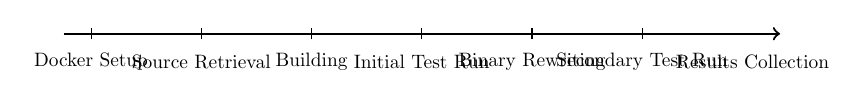
\begin{tikzpicture}[scale=0.7, every node/.style={scale=0.7}]
        \draw[->, thick] (-0.5,0) -- (12.5,0);
        
        \foreach \x in {0,2,4,6,8,10}
            \draw (\x,-0.1) -- (\x,0.1);
        
        \draw (0,-0.5) node {Docker Setup};
        \draw (2,-0.5) node {Source Retrieval};
        \draw (4,-0.5) node {Building};
        \draw (6,-0.5) node {Initial Test Run};
        \draw (8,-0.5) node {Binary Rewriting};
        \draw (10,-0.5) node {Secondary Test Run};
        \draw (12,-0.5) node {Results Collection};
    \end{tikzpicture}
    \end{center}


\textbf{Awareness of Limitations and Areas for Future Improvement}

It's crucial to acknowledge that the current iteration of RBMT, while promising, is far
from being exhaustive. Given that it was developed over a single undergraduate project
semester, it has not yet fully addressed all the challenges we've identified. However, we've
outlined several priority areas for future improvements:

\textbf{Creating Custom Docker Images (core feature):} The top priority is the development
of our own Docker images and Dockerfiles. This change will simplify the project's
onboarding process for anyone wishing to run the test suite. It will also significantly ease the
process of modifying these images and ensure transparency. Moreover, it will guarantee
that the Docker images are lean, containing only necessary packages, and are on a uniform
configuration — a crucial aspect in adhering to the scientific method.

\textbf{Expanding the Test Suite (broadening the test suite):} Currently, our test suite
includes only five subjects. Adding more subjects to the test suite, ideally approaching the
number used in GrammaTech's suite, is a key next step.

\textbf{Implementing Caching Mechanisms (optimization):} Given the extensive runtime of
the test suite, incorporating caching mechanics post-building is an area for improvement.
For instance, one could envisage bypassing the first testing phase if we have already run it
before, as we could assume that rerunning the same subject with its identical test suite will
yield consistent results. Storing the rewritten versions of the subjects could also be
beneficial, mysql for example may even take up to 7h30 in order to be fully rewritten.

\textbf{Broadening OS and Compiler Options (broadening the test suite):} The expansion
to include different operating systems and compilers would also enhance the overall
robustness and utility of the RBMT tool.

\textbf{Improving and varying the testing methods (improving depth of testing):}
Gathering more empirical data, such as execution time for each rewriter and size
comparisons between original and rewritten binaries, would provide further valuable
insights. We can also track the memory usage, CPU usage, network traffic, and system calls
as the binaries are run, as well as reimplementing fuzzing as in the GrammaTech study.
These improvements are a roadmap for the ongoing development of RBMT, moving
it closer to a comprehensive solution for binary rewriter testing and eval

%%%%%%%%%%%%%%%%%%%%
\chapter{Results}
%%%%%%%%%%%%%%%%%%%%

\begin{table}[h]
    \centering
    \caption{Success rate of Binary Rewrites with Zipr}
    \begin{tabular}{|l|l|l|l|}
    \hline
    Subject & Total & Passed & Success rate \\ \hline
    coreutils & 641 & 641 & 100.00\% \\ \hline
    coreutils (no rewrite) & 641 & 641 & 100.00\% \\ \hline
    libreoffice & 1 & 0 & 0.00\% \\ \hline
    libreoffice (no rewrite) & 1 & 1 & 100.00\% \\ \hline
    mysql & 292 & 292 & 100.00\% \\ \hline
    mysql (no rewrite) & 292 & 292 & 100.00\% \\ \hline
    redis & 90 & 89 & 98.89\% \\ \hline
    redis (no rewrite) & 90 & 89 & 98.89\% \\ \hline
    sqlite & 46386 & 46386 & 100.00\% \\ \hline
    sqlite (no rewrite) & 302151 & 302151 & 100.00\% \\ \hline
    \end{tabular}
    \end{table}
    
    \begin{table}[h]
    \centering
    \caption{Success rate of Binary Rewrites with e9patch}
    \begin{tabular}{|l|l|l|l|}
    \hline
    Subject & Total & Passed & Success rate \\ \hline
    coreutils & 641 & 640 & 99.84\% \\ \hline
    coreutils (no rewrite) & 641 & 640 & 99.84\% \\ \hline
    libreoffice & 1 & 1 & 100.00\% \\ \hline
    libreoffice (no rewrite) & 1 & 1 & 100.00\% \\ \hline
    mysql & 292 & 292 & 100.00\% \\ \hline
    mysql (no rewrite) & 292 & 292 & 100.00\% \\ \hline
    redis & 90 & 90 & 100.00\% \\ \hline
    redis (no rewrite) & 90 & 90 & 100.00\% \\ \hline
    sqlite & 302151 & 302151 & 100.00\% \\ \hline
    sqlite (no rewrite) & 302151 & 302151 & 100.00\% \\ \hline
    \end{tabular}
    \end{table}
    
    \begin{table}[h]
    \centering
    \caption{Success rate of Binary Rewrites with ddisasm}
    \begin{tabular}{|l|l|l|l|}
    \hline
    Subject & Total & Passed & Success rate \\ \hline
    coreutils & 641 & 640 & 99.84\% \\ \hline
    coreutils (no rewrite) & 641 & 641 & 100.00\% \\ \hline
    libreoffice & 1 & 0 & 0.00\% \\ \hline
    libreoffice (no rewrite) & 1 & 1 & 100.00\% \\ \hline
    mysql & N/A & N/A & N/A \\ \hline
    mysql (no rewrite) & 292 & 292 & 100.00\% \\ \hline
    redis & 90 & 89 & 98.89\% \\ \hline
    redis (no rewrite) & 90 & 90 & 100.00\% \\ \hline
    sqlite & 302151 & 302151 & 100.00\% \\ \hline
    sqlite (no rewrite) & 302151 & 302151 & 100.00\% \\ \hline
    \end{tabular}
    \end{table}
    
    \begin{table}[h]
    \centering
    \caption{Direct comparison of success rates of Binary Rewrites with all 3 studied rewriters}
    \begin{tabular}{|l|l|l|l|}
    \hline
    subject & zipr & e9patch & ddisasm \\ \hline
    coreutils & 100.00\% & 99.84\% & 99.84\% \\ \hline
    libreoffice & 0.00\% & 100.00\% & 0.00\% \\ \hline
    mysql & 100.00\% & 100.00\% & N/A \\ \hline
    redis & 98.89\% & 100.00\% & 98.89\% \\ \hline
    sqlite & 100.00\% & 100.00\% & 100.00\% \\ \hline
    \end{tabular}
    \end{table}

%%%%%%%%%%%%%%%%%%%%
\chapter{Conclusion}
%%%%%%%%%%%%%%%%%%%%

In summary, this report has introduced RBMT, a framework designed explicitly for testing binary rewriters. 
As a comprehensive platform, RBMT aims at permitting large-scale assessments of binary rewriters, while also accommodating a 
diversity of subjects within a controlled environment.

However, it is essential to note the limitations of RBMT. As it stands, RBMT can only evaluate binary rewriters on 
Linux binaries and supports a restricted range of subjects. Consequently, we anticipate future research 
endeavours that will strive to augment RBMT's capabilities by expanding its support for a broader set of subjects and architectures.

Further, as an embodiment of RBMT's potential, we conducted an analysis of three binary rewriters: Zipr, e9patch,
and ddisasm. This study served not only as a testament to RBMT's efficacy in testing binary rewriters but also 
highlighted its aptitude in quantifying their performance. Therefore, this exploration reaffirms our belief in 
RBMT as an instrumental tool in the realm of binary rewriting evaluation, signaling promising possibilities for
its future development.

\cleardoublepage
\phantomsection
\addcontentsline{toc}{chapter}{Bibliography}
\printbibliography

% Appendices are optional
% \appendix
% %%%%%%%%%%%%%%%%%%%%%%%%%%%%%%%%%%%%%%
% \chapter{How to make a transmogrifier}
% %%%%%%%%%%%%%%%%%%%%%%%%%%%%%%%%%%%%%%
%
% In case you ever need an (optional) appendix.
%
% You need the following items:
% \begin{itemize}
% \item A box
% \item Crayons
% \item A self-aware 5-year old
% \end{itemize}

\end{document}